\chapter{动力系统}
\label{cha:Motor}

\section{双极型步进电机}

Bipolar motors

\url{https://en.wikipedia.org/wiki/Stepper_motor}

\begin{figure}[htbp]
    \centering
    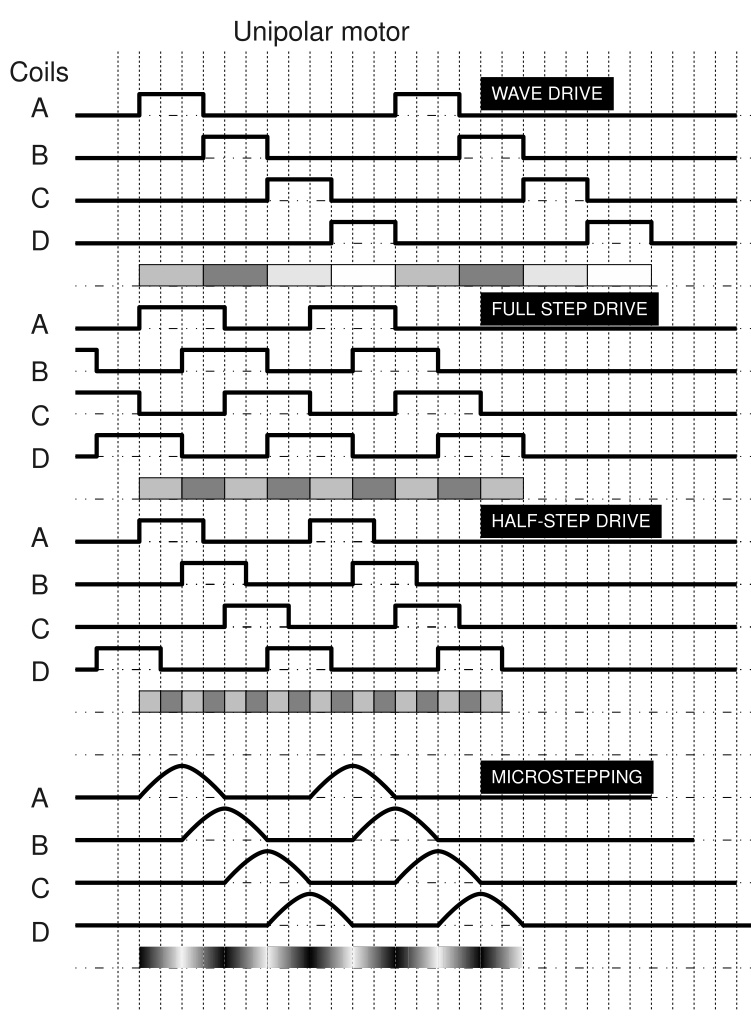
\includegraphics[width=\columnwidth]{Drive.png}
    \caption{Phase current waveforms}
    \label{fig:Phase-current}
\end{figure}

双极电动机每相只有一个绕组。为了使磁极反向,需要使绕组中的电流反向,因此驱动电路必须更复杂,通常采用H桥配置(但是有几种现成的驱动器芯片可以使之成为一个简单的事情)。每相有两个引线,没有公用的。

两线圈双极步进电动机的典型驱动模式为:A + B + A- B-。即以正电流驱动线圈A,然后从线圈A中去除电流。然后以正电流驱动线圈B,然后从线圈B中去除电流。然后用负电流驱动线圈A(通过切换导线,例如用H桥翻转极性),然后从线圈A去除电流。然后用负电流驱动线圈B(与线圈A的翻转极性相同);循环完成并重新开始。

由于更好地利用了绕组,因此它们比同等重量的单极电动机更强大。这是由于绕组占用的物理空间。单极电机在相同的空间中具有两倍的导线数量,但在任何时间点仅使用一半的导线,因此效率为50\%(或大约70\%的可用扭矩输出)。尽管双极步进电机的驱动更加复杂,但丰富的驱动芯片简化了实际使用时的复杂度。

\section{步进电机驱动}

斩波驱动电路(Chopper drive circuits)称为受控电流驱动器,因为它们在每个绕组中产生受控电流,而不是施加恒定电压。斩波器驱动电路最常用于双绕组双极电动机,两个绕组被独立驱动以提供特定的电动机转矩CW或CCW。在每个绕组上,将“电源”电压作为方波电压施加到绕组上。例如8 kHz。绕组电感使电流平滑,该电流达到根据方波占空比的水平。相对于绕组回路,双极性电源(+和-)电压通常提供给控制器。

\section{步进电机驱动DRV8825}

\begin{figure}[htbp]
    \centering
    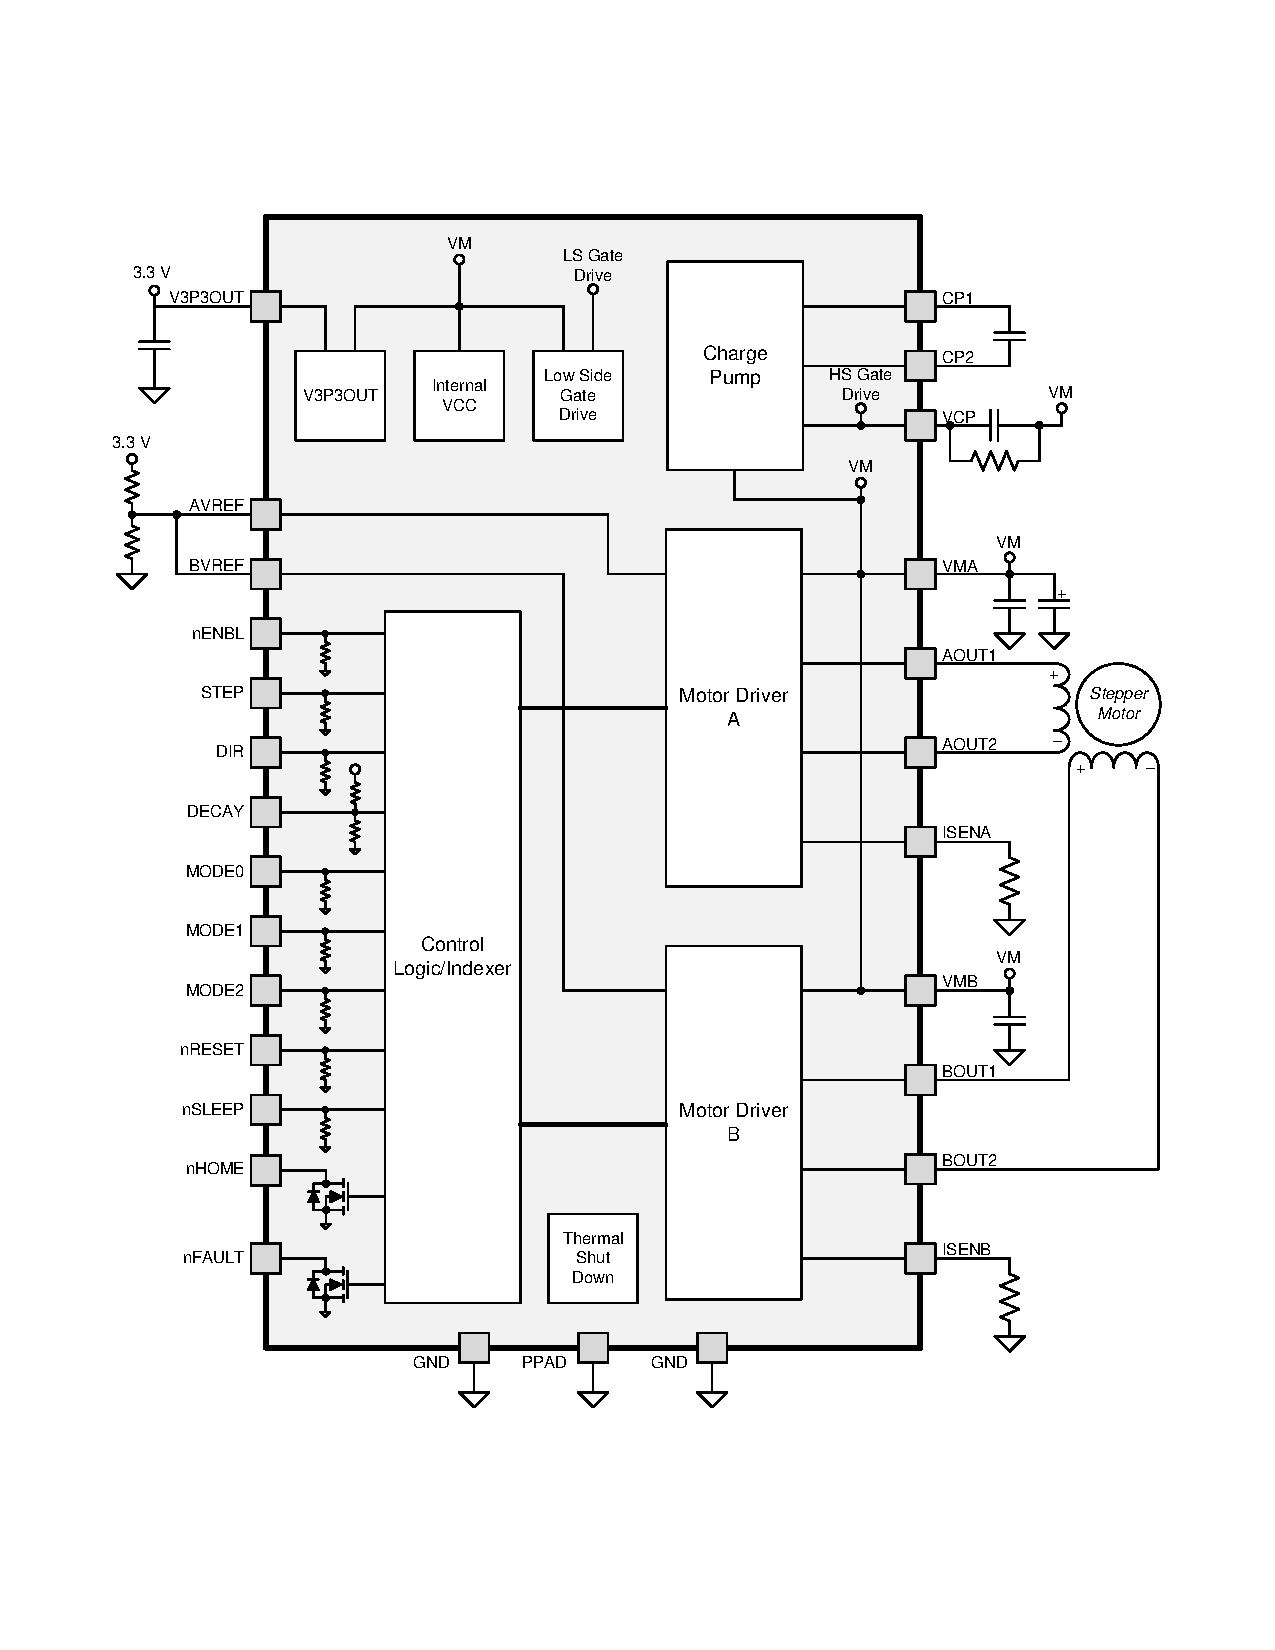
\includegraphics[width=\columnwidth]{DRV8825-Function-Block.pdf}
    \caption{DRV8825功能框图}
    \label{fig:DRV8825-Function-Block}
\end{figure}
